\chapter{Results and Discussion}
\label{chp:results_and_discussion}

\lettrine{O}{utcomes} of each simulation experiment are presented. The performance of the guidance law is assessed based on performance in the numerical experiments. Consideration of the methodology is used to explain some of the observed behaviours, and deficiencies are noted for improvement.

\section{Baseline Case Runs}
The baseline trajectory cases outlined in Tables \ref{tab:trajectory_cases} and \ref{tab:trajectory_case_params} were simulated, and the main results are shown in Table \ref{tab:outputs_1_summary}.
\begin{table}[H]
  \centering
  \begin{tabular}{lR{3cm}R{2.5cm}rr}
    \toprule
    \textbf{Case ID} & Convergence Tolerance & Time of Flight (d) & \# Revolutions & CPU Time (s) \\
    \midrule
    A                & 0.001                 & 621                & 862            & 17.6         \\
    B                & 0.03                  & 498                & 501            & 16.9         \\
    C                & 0.005                 & 802                & 1560           & 38.3         \\
    D                & 0.005                 & 63                 & 62             & 10.1         \\
    \bottomrule
  \end{tabular}
  \caption{Summary of outcomes for each case.}
  \label{tab:outputs_1_summary}
\end{table}

Case-by-case plots of the time history of the orbital elements and the spatial trajectory are shown below.
\subsection{Plots: Case A}
\begin{figure}[H]
  \centering
  \begin{subfigure}[t]{0.4\textwidth}
    \includegraphics[width=\textwidth]{figures/benchmark_transfer/orbital_elements.pdf}
    \caption{Evolution of orbit elements in time.}
    \label{fig:results_a_a}
  \end{subfigure}
  \begin{subfigure}[t]{0.59\textwidth}
    \includegraphics[width=\textwidth]{figures/benchmark_transfer/trajectory_plot.png}
    \caption{Trajectory plot.}
    \label{fig:results_a_b}
  \end{subfigure}
  \caption{Orbital elements and trajectory for case A.}
  \label{fig:results_a}
\end{figure}

\subsection{Plots: Case B}
\begin{figure}[H]
  \centering
  \begin{subfigure}[t]{0.4\textwidth}
    \includegraphics[width=\textwidth]{figures/oguri_G/orbital_elements.pdf}
    \caption{Evolution of orbit elements in time.}
    \label{fig:results_results_b_a}
  \end{subfigure}
  \begin{subfigure}[t]{0.59\textwidth}
    \includegraphics[width=\textwidth]{figures/oguri_G/trajectory_plot.png}
    \caption{Trajectory plot.}
    \label{fig:results_results_b_b}
  \end{subfigure}
  \caption{Orbital elements and trajectory for case B.}
  \label{fig:results_results_b}
\end{figure}

\subsection{Plots: Case C}
\begin{figure}[H]
  \centering
  \begin{subfigure}[t]{0.4\textwidth}
    \includegraphics[width=\textwidth]{figures/plane_change/orbital_elements.pdf}
    \caption{Evolution of orbit elements in time.}
    \label{fig:results_c_a}
  \end{subfigure}
  \begin{subfigure}[t]{0.59\textwidth}
    \includegraphics[width=\textwidth]{figures/plane_change/trajectory_plot.png}
    \caption{Trajectory plot.}
    \label{fig:results_c_b}
  \end{subfigure}
  \caption{Orbital elements and trajectory for case C.}
  \label{fig:results_c}
\end{figure}

\subsection{Plots: Case D}
\begin{figure}[H]
  \centering
  \begin{subfigure}[t]{0.4\textwidth}
    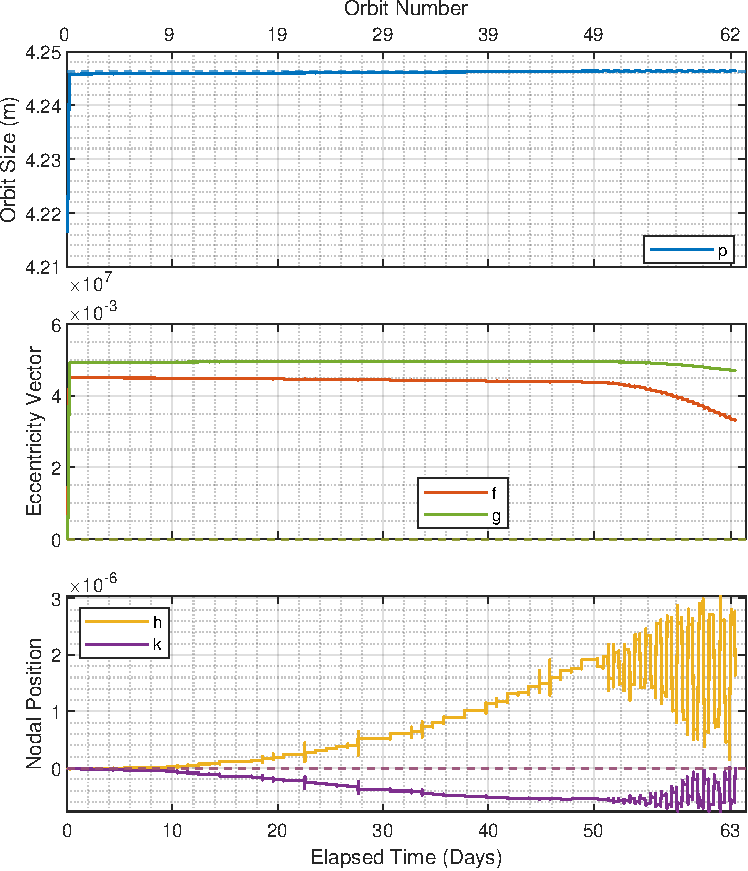
\includegraphics[width=\textwidth]{figures/geo_disposal/orbital_elements.pdf}
    \caption{Evolution of orbit elements in time.}
    \label{fig:results_results_c_a}
  \end{subfigure}
  \begin{subfigure}[t]{0.59\textwidth}
    \includegraphics[width=\textwidth]{figures/geo_disposal/trajectory_plot.png}
    \caption{Trajectory plot.}
    \label{fig:results_results_c_b}
  \end{subfigure}
  \caption{Orbital elements and trajectory for case D.}
  \label{fig:results_results_c}
\end{figure}

\subsection{Animations: Cases A-C}
Note: a javascript-enabled PDF reader (e.g. Adobe Reader, Foxit Reader) is required for view the animations. Seeing the trajectories animated in 3D space may help provide a more comprehensible view of what is going on.

\begin{figure}[H]
  \animategraphics[width=\textwidth, controls, loop]{10}{animations/benchmark_transfer/anim-}{1}{50}
  \caption{Trajectory animation for case A.}
  \label{fig:anim_a}
\end{figure}

\begin{figure}[H]
  \animategraphics[width=\textwidth, controls, loop]{10}{animations/oguri_case_G/anim-}{1}{47}
  \caption{Trajectory animation for case B.}
  \label{fig:anim_b}
\end{figure}

\begin{figure}[H]
  \animategraphics[width=\textwidth, controls, loop]{10}{animations/plane_change/anim-}{1}{50}
  \caption{Trajectory animation for case C.}
  \label{fig:anim_c}
\end{figure}



Overall, it is evident that despite being convergent, the guidance law is extremely slow at advancing the orbit in certain segments.

The low thrust produced by the sail is not the key issue; rather, it is the lack of availability of thrust in a given direction. For example, a continuous thrust plane change maneuver involves continuously changing the direction of applied thrust. The direction desired by the first stage of the guidance law is not always available, and the solar sail often ends up being feathered (this effect has not yet been quantified; pending measurement of time spent in degraded/feathered operational mode).

Part of the issue with the long time of flight is the convergence tolerance (measured as the sum of the squares of the error in each element, weighed by \(W_{\moe}\); this will be changed to the value of \(Q\) in the future). The guidance law can reach an error of about 0.05 reasonably quickly, but spends a substantial amount of time finely correcting its trajectory at the end, resulting in very slow convergence to the final threshold.

For initial orbits very close to the target orbit (e.g. GEO disposal case), the guidance law struggles with closing the gap, and often results in extremely long missions. Altering guidance weights helps with this somewhat (see the guidance weights of the GEO disposal case, for example), but it is currently unknown whether there are also numerical artifacts to consider.

More insights are evident through inspection of the plots of the trajectory and orbital elements. Discussion on these is presented in the next section.

\section{Global Optimization Runs}
Global weight optimization was performed for the latter two baseline cases. The optimized guidance law tunings are compared against their unoptimized counterparts in Table \ref{tab:outputs_2_summary}.

\begin{table}[H]
  \centering
  \begin{tabular}{L{5cm}L{2.5cm}L{2.5cm}L{3cm}}
    \toprule
    \textbf{Case}                                     & Time of Flight (d) & Number of Revolutions & \(\Delta v\) Expenditure (m/s) \\
    \midrule
    ``Benchmark'', baseline                           & 610                & 858                   & 6673.2                         \\
    \rowcolor{green!20!white}``Benchmark'', optimized & 388                & 622                   & 6193.0                         \\
    Polar GSO, baseline                               & 490                & 494                   & 9686.7                         \\
    \rowcolor{green!20!white} Polar GSO, optimized    & 375                & 323                   & 8352.0                         \\
    \bottomrule
  \end{tabular}
  \caption{Comparison of optimized cases against their baselines.}
  \label{tab:outputs_2_summary}
\end{table}

The two cases still use their original convergence tolerances in the optimized tunings.

Plots of the trajectories and orbital elements are shown in Sections \ref{sec:bench_case_plot} and \ref{sec:gso_case_plot}.

\subsection{Benchmark Case}
\label{sec:bench_case_plot}
Baseline \(W_{\moe}\): \(\{1, 1, 1, 1, 1\}\)


Optimal \(W_{\moe}\): \(\{1.774, 0.5149, 0.3327, 9.925, 0.5317\}\)

\begin{figure}[H]
  \centering
  \begin{subfigure}[t]{0.49\textwidth}
    \includegraphics[width=\textwidth]{figures/benchmark_optim/orbital_elements.pdf}
    \caption{Evolution of orbit elements in time.}
    \label{fig:results_benchmark_optim_a}
  \end{subfigure}
  \begin{subfigure}[t]{0.49\textwidth}
    \includegraphics[width=\textwidth]{figures/benchmark_optim/trajectory_plot.png}
    \caption{Trajectory plot.}
    \label{fig:results_benchmark_optim_b}
  \end{subfigure}
  \caption{Benchmark transfer case, optimal tuning.}
  \label{fig:results_benchmark_optim}
\end{figure}


\begin{figure}[H]
  \begin{animateinline}[controls,width=\linewidth, loop]{10}
    \multiframe{50}{i=1+1}{
      \includegraphics[height=0.5\textwidth]{animations/benchmark_transfer/anim-\i}%
      \includegraphics[height=0.5\textwidth]{animations/benchmark_transfer_optim/anim-\i}}
  \end{animateinline}
  \caption{Benchmark transfer before/after optimization (use Adobe Reader to view the animations.)}
  \label{fig:benchmark_optim_anim}
\end{figure}
% View: -70, 20

\newpage
\subsection{Polar GSO Case}
\label{sec:gso_case_plot}
Baseline \(W_{\moe}\): \(\{1, 1, 1, 1, 1\}\)
\begin{figure}[H]
  \centering
  \begin{subfigure}[t]{0.49\textwidth}
    \includegraphics[width=\textwidth]{figures/oguri_G/orbital_elements.pdf}
    \caption{Evolution of orbit elements in time.}
    \label{fig:oguri_base_a}
  \end{subfigure}
  \begin{subfigure}[t]{0.49\textwidth}
    \includegraphics[width=\textwidth]{figures/oguri_G/trajectory_plot.png}
    \caption{Trajectory plot.}
    \label{fig:oguri_base_b}
  \end{subfigure}
  \caption{GTO to polar transfer, baseline.}
  \label{fig:oguri_base}
\end{figure}

Optimal \(W_{\moe}\): \(\{8.959, 2.132, 1.722, 3.559, 9.789\}\)

\begin{figure}[H]
  \centering
  \begin{subfigure}[t]{0.49\textwidth}
    \includegraphics[width=\textwidth]{figures/oguri_optim/orbital_elements.pdf}
    \caption{Evolution of orbit elements in time.}
    \label{fig:oguri_optim_a}
  \end{subfigure}
  \begin{subfigure}[t]{0.49\textwidth}
    \includegraphics[width=\textwidth]{figures/oguri_optim/trajectory_plot.png}
    \caption{Trajectory plot.}
    \label{fig:oguri_optim_b}
  \end{subfigure}
  \caption{GTO to polar transfer, optimal tuning.}
  \label{fig:oguri_optim}
\end{figure}

\section{Discussion}

The improvement in time-of-flight (and number of revolutions) is remarkable. By inspecting the plots of the orbital elements, it is clear that adjusting the weights of the guidance changes the ``strategy'' employed by the guidance law.

By emphasizing certain elements over others, the guidance law is more willing to accept an increase in error in one element for a reduction in another. This is exemplified in Figure \ref{fig:results_benchmark_optim_a}.

By inspecting the trajectory plots, it is evident that the optimized transfers ``waste fewer actions'' compared to their baseline counterparts. In the Benchmark case, the total \(\Delta v\) expenditures are very similar, but the trajectory taken by the optimized tuning looks far more direct than the baseline case.




\section{Validity of Methodology}

\begin{itemize}
  \item NEed more baseline Cases
  \item Restricted solar sail angle study is kinda bunk
\end{itemize}